\documentclass[12pt]{article}
\usepackage[utf8]{inputenc}
\usepackage[a4paper]{geometry}
\usepackage[utf8]{inputenc}
\usepackage[english]{babel}
\usepackage{wrapfig}
\usepackage{graphicx}
\usepackage{listings}
\usepackage{biblatex}
\addbibresource{bibliography.bib}

\title{Report in \LaTeX}
\date{August 25, 2020}
\author{Raymond Wang - 
\url{raymondw@kth.se}}

\begin{document}
\maketitle
\tableofcontents

\newpage 
\section{FEM-analysis of the thoracic aorta}

\begin{wrapfigure}{r}{0.55\textwidth}
\centering
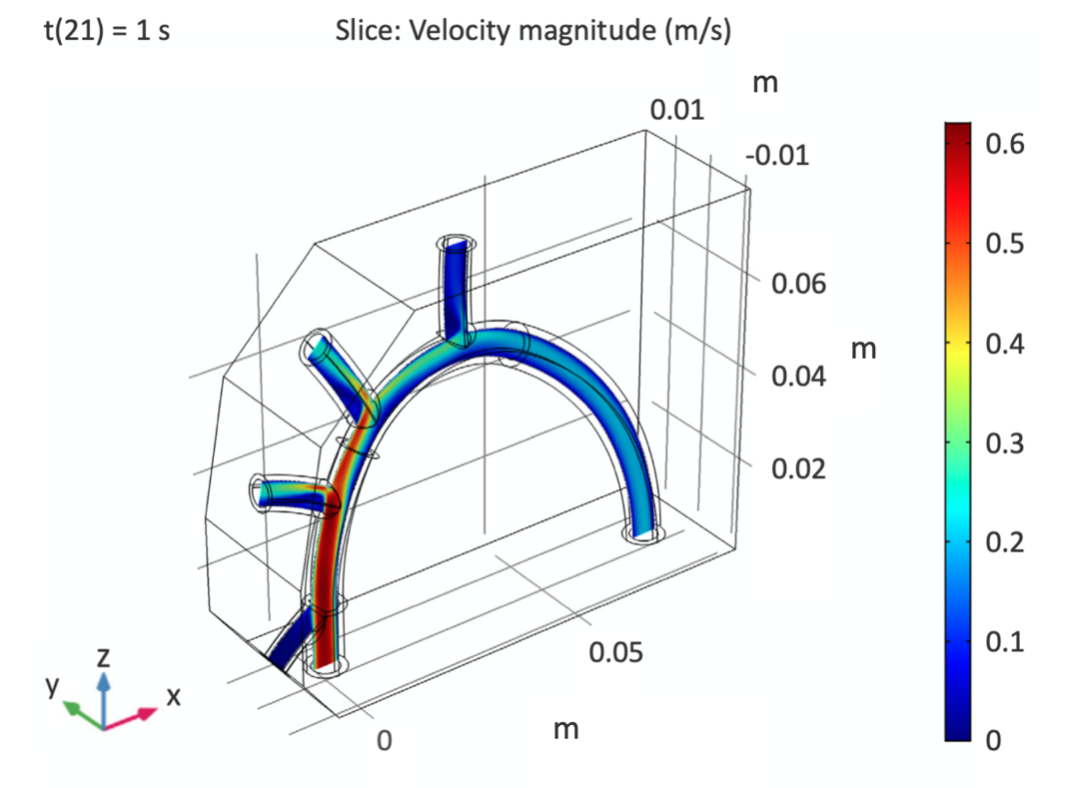
\includegraphics[width=.98\linewidth]{velocity}
\caption{Velocity magnitudes}
\end{wrapfigure}

The fluid dynamics simulation yielded the figure attached below. 
As can be noted, maximum fluid velocity is measured in the vicinity of the inlet 
while decreasing as it spreads out. Similar appearances should pertain to 
the pressure field due to direct proportionality between fluid pressure 
and velocity as stated by the Hagen–Poiseuille equation (1).

\begin{equation}
    \Delta p = \frac{8\mu LQ}{\pi R^{4}} = \frac{8 \pi LQ}{A^{2}}
\end{equation}

\noindent where: 
\begin{itemize}
    \item[] $\Delta p$ is the pressure difference between the two ends,
    \item[] $L$ is the length of pipe, \hspace{0.2cm} $Q$  is the volumetric flow rate,
    \item[] $\mu$ is the dynamic viscosity,
    $R$ is the pipe radius,
    \item[] $Q$  is the volumetric flow rate,
    $A$ is the cross section of pipe \cite{vogel2020life}.
\end{itemize}

\section{Bash command history}
\begin{lstlisting}
	raymondw@student-shell-1:~/dataintro20$ history
	1  cd dataintro20
	2  mkdir dataintro20
	3  man
	4  man
	5  ls
	6  man bash
	7  dataintro20
	8  cd dataintro20
\end{lstlisting}

\vspace{0.2cm}
\section{References}
\printbibliography[heading=none]
\end{document}
